\documentclass[tikz,border=10pt]{standalone}

\usepackage{amsmath,amsthm,amssymb,slashed,upgreek,url,graphicx}
\usepackage{mathtools,nccmath}

\usepackage{physics}
\usetikzlibrary{decorations.pathmorphing}
    % this is for graphics. e.g. rectangle on title page
\usetikzlibrary{3d}
\usetikzlibrary{backgrounds}
\usetikzlibrary{arrows,shapes,positioning,shadows,trees,mindmap}
\usetikzlibrary{tikzmark}
\usetikzlibrary{calc,math}

\usepackage{tikz-3dplot}
\usepackage{pgfplots}
\pgfplotsset{compat = newest}
%\usepgfplotslibrary{colormaps}
\usepgflibrary{shapes.geometric}

\usepackage[edges]{forest}
\usetikzlibrary{arrows.meta}
\colorlet{linecol}{black!75}
\usepackage{xkcdcolors} % xkcd colors

\usetikzlibrary{patterns}
\tikzset{>={Stealth[inset=0pt,angle=20:10pt]}}


\tikzset{zigzag/.style={decorate,decoration=zigzag}}


\begin{document}
\tikzset{every picture/.style={line width=0.75pt}} %set default line width to 0.75pt        

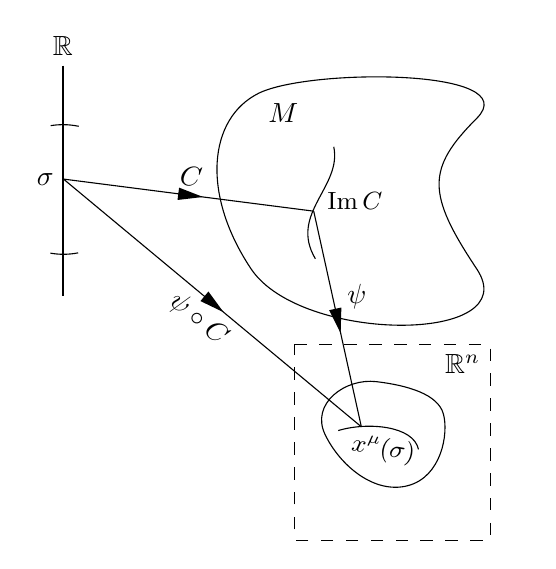
\begin{tikzpicture}[x=0.75pt,y=0.75pt,yscale=1,xscale=1]
%uncomment if require: \path (0,300); %set diagram left start at 0, and has height of 300

%Shape: Polygon Curved [id:ds15513429185302652] 
\draw   (137.46,221.39) node[below right]{$M$}.. controls (161.62,233.47) and (266.72,233.47) .. (242.56,209.31) .. controls (218.4,185.15) and (218.4,173.07) .. (242.56,136.83) .. controls (266.72,100.59) and (158,100.59) .. (133.84,136.83) .. controls (109.68,173.07) and (113.3,209.31) .. (137.46,221.39) -- cycle ;
%Straight Lines [id:da215115271864053] 
\draw    (43.24,234.68) node[above]{$\mathbb R$} -- (43.24,123.54) ;
%Curve Lines [id:da6660300067204521] 
\draw    (164.84,141.66) .. controls (151.96,163.4) and (177.73,176.29) .. (173.7,195.62) node[midway,right]{\small $\Im C$};
%Straight Lines [id:da8555715774924406] 
\draw    (43.48,180.07) node[left]{$\sigma$} -- (164.04,164.61) node[midway,sloped,above]{$C$};
\draw [shift={(110.7,171.45)}, rotate = 172.69] [fill={rgb, 255:red, 0; green, 0; blue, 0 }  ][line width=0.08]  [draw opacity=0] (12,-3) -- (0,0) -- (12,3) -- cycle    ;
%Shape: Polygon Curved [id:ds020442850645846056] 
%\draw   (163.07,204.72) .. controls (174.55,208.95) and (192.43,196.62) .. (195.08,187.2) .. controls (197.74,177.78) and (198.95,154.1) .. (191.46,142.02) .. controls (183.97,129.94) and (154.01,134.29) .. (147.01,149.03) .. controls (140,163.77) and (151.6,200.49) .. (163.07,204.72) -- cycle ;
%Straight Lines [id:da7992098944042878] 
\draw    (43.48,180.07) -- (186.99,60.73) node[midway,sloped,below]{$\psi\circ C$};
\draw [shift={(120.62,115.92)}, rotate = 140.25] [fill={rgb, 255:red, 0; green, 0; blue, 0 }  ][line width=0.08]  [draw opacity=0] (12,-3) -- (0,0) -- (12,3) -- cycle    ;
%Straight Lines [id:da48705876559434613] 
\draw    (164.04,164.61) -- (186.99,60.73) node[midway,above right]{$\psi$};
\draw [shift={(177.02,105.83)}, rotate = 102.46] [fill={rgb, 255:red, 0; green, 0; blue, 0 }  ][line width=0.08]  [draw opacity=0] (12,-3) -- (0,0) -- (12,3) -- cycle    ;
%Shape: Rectangle [id:dp46520262671682056] 
\draw  [dash pattern={on 4.5pt off 4.5pt}] (154.78,100.19) -- (249,100.19)node[below left]{$\mathbb R^n$} -- (249,5.96) -- (154.78,5.96) -- cycle ;
%Shape: Polygon Curved [id:ds019123595344816557] 
\draw   (194.24,82.47) .. controls (209.34,80.66) and (223.83,76.43) .. (226.49,67.01) .. controls (229.15,57.58) and (225.65,36.57) .. (209.34,32.34) .. controls (193.03,28.11) and (176.48,42.36) .. (169.47,57.1) .. controls (162.47,71.84) and (179.14,84.28) .. (194.24,82.47) -- cycle ;
%Curve Lines [id:da0671877791027502] 
\draw    (175.86,58.91) .. controls (189.75,63.14) and (212.1,61.33) .. (214.51,49.85) node[midway,sloped,below]{\small $x^\mu (\sigma)$};
%Shape: Arc [id:dp38552699071390983] 
\draw  [draw opacity=0] (37.29,205.8) .. controls (39.23,206.12) and (41.21,206.29) .. (43.24,206.29) .. controls (45.84,206.29) and (48.37,206.01) .. (50.81,205.5) -- (43.24,170.05) -- cycle ; \draw   (37.29,205.8) .. controls (39.23,206.12) and (41.21,206.29) .. (43.24,206.29) .. controls (45.84,206.29) and (48.37,206.01) .. (50.81,205.5) ;  
%Shape: Arc [id:dp4430004713949758] 
\draw  [draw opacity=0] (50.57,144.53) .. controls (48.3,144.08) and (45.96,143.84) .. (43.56,143.84) .. controls (41.38,143.83) and (39.25,144.02) .. (37.17,144.38) -- (43.48,180.07) -- cycle ; \draw   (50.57,144.53) .. controls (48.3,144.08) and (45.96,143.84) .. (43.56,143.84) .. controls (41.38,143.83) and (39.25,144.02) .. (37.17,144.38) ;  
\end{tikzpicture}
\end{document}